%%%%%%%%%%%%%%%%%%%%%%%%%%%%%%%%%%%%%%%%%%%%%%%%%%%%%%%%%%%%%%%%%%%
%                                                                 %
%                            CHAPTER FOUR                          %
%                                                                 %
%%%%%%%%%%%%%%%%%%%%%%%%%%%%%%%%%%%%%%%%%%%%%%%%%%%%%%%%%%%%%%%%%%%
\chapter{Recognition} \label{sec:recognition}
This chapter reviews in detail the primary contributions of this thesis: the recognition, fitting, and classification of objects in the new sketching interface. The recognition of objects refers to the system's awareness to the presence of a series of strokes representing an object. Object fitting results in a generated shape that accurately represents an object recognized by the system. Lastly, the classification of an object results in the designation of certain attributes determined by its physical properties. These application features use and build from the metrics described in chapter 3.  These components elevate the sketching interface beyond a simple painting program. The system is intended to recognize the input, understand the user's intentions and reiterate that to the user an image that is meaningful and easy to understand. \\

\begin{figure}[ht]
\centering
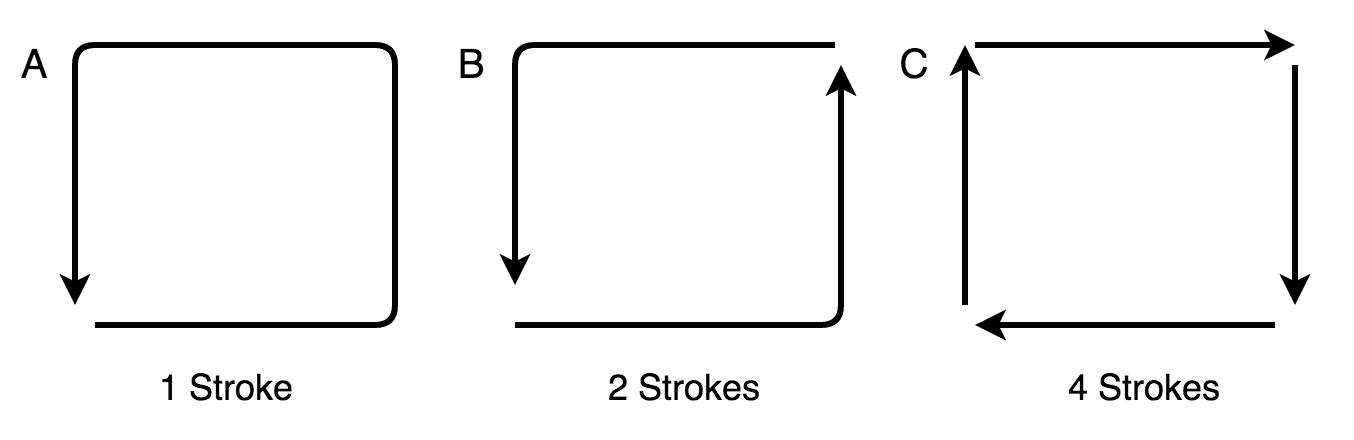
\includegraphics[width=\textwidth]{multistrokes}
\caption[Comparisons between methods of drawing a rectangle using different amounts of lines.]{Illustrated are methods of drawing a rectangle using different amounts of lines. This application currently only recognizes rectangles drawn with four strokes.}
\label{fig:multistrokes}
\end{figure}

Due to the shapes of objects we currently allow in OASIS, all objects may be accurately represented in 2D as a rectangle. Therefore, the algorithms presented are specialized to solve for the subset of shapes similar to rectangles. The problem set is further simplified to recognize only sets of straight lines that are of size 4. However, proposed methods to overcome this limitation will be presented. \\

I present a geometric based approach to recognizing rectangles from user drawn lines. The basic features of a rectangle were analyzed to create metrics useful in determining the existence of a user drawn rectangle. Since multiple rectangles may be created from a common set of strokes, scoring functions are necessary in determining the optimal outcome. Algorithms and analysis for primary scoring functions are displayed and evaluated. Afterwards, in section \ref{sec:classification}, I present a method to classify rectangles based on their attributes. Finally, we will discuss my approach to fit a rectangle to a set of user drawn strokes in section \ref{sec:rectfitting}. \\

\section{Recognition Pipeline}
\label{sec:recognitionpipeline}
%talk about the pipeline at a high level
As discussed briefly in the previous chapter, the last step of the overall system pipeline is the recognition process. The pipeline of the recognition process is illustrated in Figure \ref{fig:sketchpipeline}. The recognition process contains the steps needed to recognize, fit, and classify objects based on user created strokes. To begin, the system creates certain combinations of strokes, using all of the user generated data points to determine which strokes match best with others. Using the generated combinations, the interface scores those groupings of strokes based on a number of metrics. If any combinations exceed a certain confidence level, then that set of strokes is deemed to be a possible object. \\

\begin{figure}[ht]
\centering
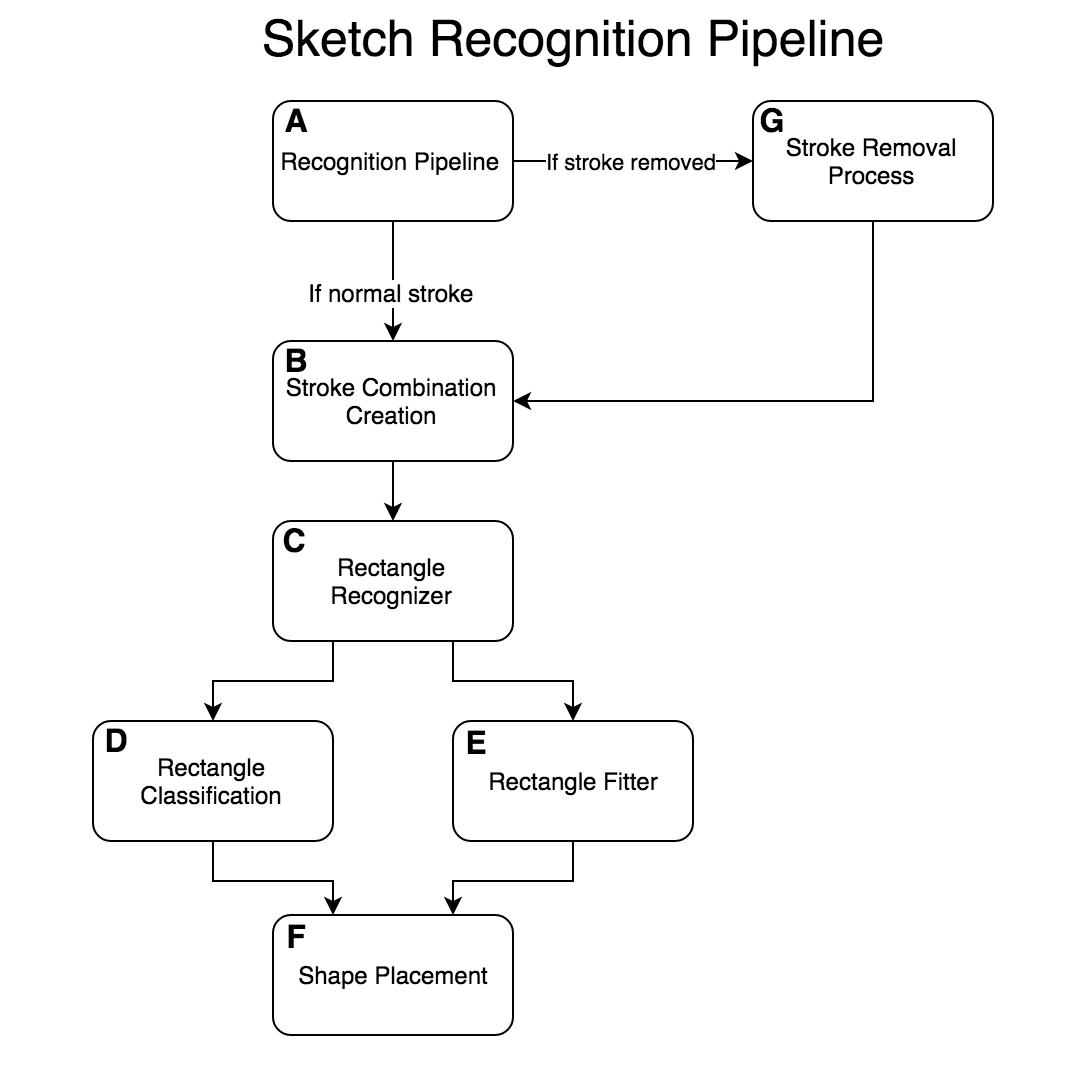
\includegraphics[width=.9\textwidth]{sketchpipeline}
\caption[Recognition pipeline diagram]{Simplified diagram outlining the steps to recognize rectangles from a set of strokes.}
\label{fig:sketchpipeline}
\end{figure}

Once the system has obtained a list of the combinations of strokes that have been accepted as rectangles, it selects the series of objects yielding the highest score to be drawn onto the interface. Afterwards, the chosen sets of strokes are assessed using two algorithms: one for fitting the best possible rectangle, and one for an initial classification type. We attempt to fit rectangles to the user's drawn strokes in order to display our interpretation of the design. The fitting uses a 2D heuristic created from the sum of the overall distance from the proposed rectangle to each one of the points from the user created strokes. Next, a classification algorithm from the system presents the user with an initial type for the newly created object. Finally, the shape is placed on the screen for the user to evaluate and edit. After the conclusion of this pipeline, the user may continue to engage with the interface, repeating the pipeline for each stroke added. Or, the user may conclude editing, which continues onto the rest of the OASIS processes.

%the thought process behind the steps?
%combinations of 4
%why only 4
%how do we pick them
%math of scoring
%angle and distance

\section{Combinations of Strokes}
\label{sec:combostrokes}

While it is possible to generate the score of all subsets given all user strokes, scoring $2^n$ combinations of strokes is inefficient. Also, choosing random sets of strokes does not ensure a sufficient level of accuracy. I propose a scoring algorithm to select particular groupings that maximize the probability of the strokes forming a coherent rectangle. \\

To begin, each stroke is compared with every other stroke. As shown in Equation \ref{equ:comboscoring}, the score between two strokes is determined by their interior angle between the two lines and their distance apart. Each score is recorded and new scores are calculated only when a new stroke is produced by the user or an existing stroke is edited. \\

As shown in Equation \ref{equ:perpendicular}, the \textit{perpendicular} equation penalizes strokes that are not perpendicular with one another. The angles are calculated using the the line of best fit algorithm described in the section \ref{sec:bestfit}. An angle that is a multiple of 45 (but not 90) produces the highest score. A low score indicates a better fit (more similar) to the original stroke.

\begin{equation}
\label{equ:perpendicular}
perpendicular(x,y) = \dfrac{45 - |((x_{angle} - y_{angle})\%90) - 45|}{45}
\end{equation}

The \textit{distance} equation, as shown in Equation \ref{equ:dist}, rewards pairs of strokes with small amounts of distance between them. Distance between two strokes is measured by the smallest Euclidean distance between all combinations of the strokes' endpoints. Nearby and perpendicular strokes represent the types most likely to form a rectangle with one another.

\begin{equation}
\label{equ:dist}
distance(x,y) = \dfrac{endPointDistance(x,y)}{max(canvas_{w}, canvas_{h})}
\end{equation}

The two metrics are summed to create a score representing the probability that two strokes are likely to form a rectangle with one another. A low score represents a high probability of rectangle cohesion, while a high score implies a low probability. Using each stroke's list of scores against all other strokes, we pick from the top scoring strokes to create sets of four for the next process in the recognizer.

\begin{equation}
\label{equ:comboscoring}
Score(x,y) = perpendicular(x,y) + distance(x,y)
\end{equation}

% For each stroke that is added by the user, it is scored against all other strokes. Each stroke records its score against all other strokes in a priority queue. The stroke will later use the top scoring neighboring strokes to create groupings, avoiding other strokes it was unlikely to create an object with.  Ideally, the first 3 strokes will be popped from the queue, and combine with the base stroke to create an object. \\

%SIMILARLITY CHECK
% The before mentioned metrics would allow strokes that are virtually identical score extremely well. However, a rectangle representing a furniture item will rarely contain 2 strokes that are visually the same in both angle and position. Therefore, pairs of strokes scoring below .05 will not be considered. \\

I acknowledge that not all rectangles created by users are created with 4 strokes. However, the metrics needed to define a rectangle drawn with 1, 2, or $n$ strokes adds a new level of complexity to the problem. With any numbers other than 4, the strokes would need to be normalized to 4 with some method. For numbers less than 4, I propose breaking strokes at their corners. For numbers greater than 4, a method to combine similar lines would be needed.

\section{Rectangle Recognizer}
\label{sec:rectrecognizer}

%aka how do we know four strokes are a rectangle, etc.
To recognize a set of strokes as a rectangle, the recognizer works in three basic steps: rejecting groupings that do not pass the threshold for the rectangle metrics, scoring the groups of strokes that do exceed the threshold, and selecting the top scoring groupings as an object. The rectangle metrics are three heuristics that, when passed in conjunction, almost always produce a recognizable rectangle. Even if a stroke belongs to more than one possible set, it may only form an object with the highest scoring set of strokes where all other members do not belong to any higher scoring group. Given a large set of possible combinations, the recognizer selects the best to be created into rectangles.
%choosing of the 4 strokes

%the three checks
\subsection{Rectangle Metrics}
%all are close to lines
%reference the line algorithm from before

This subsection lists and describes the metrics used to identify if a set of strokes is mathematically similar to a rectangle.

\subsubsection{Line Ending Comparison}

The first rectangle metric specifies that all stroke endpoints in the set must be near another unique endpoint within the same set. This metric ensures that the strokes are spatially adjacent and create a closed polygon.

%line ending pairings
\begin{algorithm}
\caption[Function for Line Ending Pairings]{Function detailing the pairings of line endings}
\label{alg:lineendings}
\begin{algorithmic}[1]
\Function{LineEndings}{endPoints, maxDist}
\State $pairs \gets $ []
\For{$i = 0 \to $\textbf{sizeof}$ endPoints - 1 $ }
    \For{$j = i+1  \to$ \textbf{sizeof}($ endPoints $) }
        \State $d \gets distance(endPoints_i, endPoints_j)$
        \If{$d < maxDist$}
            \State $pairs \gets [endPoints_i, endPoints_j]$
            \State \textbf{remove} $i, j$
            \State \textbf{break}
        \EndIf
    \EndFor
    \If{\textbf{sizeof}($pairs$) $<$ \textbf{sizeof}($endPoints$)/2}
        \State \textbf{return} []
    \Else
        \State \textbf{return} pairs
    \EndIf
\EndFor
\EndFunction
\end{algorithmic}
\end{algorithm}

Algorithm \ref{alg:lineendings} outlines the greedy method used to pair the line endings. Endpoints are compared by distance and paired with the first choice within the maximum distance allowed.

\begin{equation}
\label{equ:maxdistcorners}
maxDist = \dfrac{p}{n} \cdot \sum_{i=0}^{n-1} length(stroke_i)
\end{equation}

Equation \ref{equ:maxdistcorners} describes a formula to determine the maximum distance allowed between endpoint pairings given $n$ strokes and percentage of stroke length $p$. I used a percentage of .1, the desired maximum distance between endpoints was 10 percent of the average length of strokes involved. 

\subsubsection{Line Straightness}
The second rectangle metric states that all strokes in a rectangle object must be similar in straightness to a line. To determine this, I use the LengthRatio described in Equation \ref{equ:ratio3}. The purpose of this metric is to ensure there exists no odd edges or irregularities; a wavy line will receive a poor score when comparing similarity against the straight edge of a rectangle. While I did use .95 as a threshold for a line when sketching walls, I used a .9 threshold for this metric to allow for a little more flexibility.

\subsubsection{Perpendicular Angles}

A property of all rectangles is that all interior angles equal 90 degrees. Therefore, the last rectangle metric is the average interior angle of the set of strokes.\\

\begin{equation}
\label{equ:angle2strokes}
\theta = tan(\dfrac{|slope_i - slope_{j}|}{1 + (slope_i \cdot slope_{j})})
\end{equation}

\begin{equation}
\label{equ:center}
\begin{aligned}
center_x = \dfrac{1}{n} \cdot \sum_{i=0}^{n} stroke_i.x
\\[1pt]
center_y = \dfrac{1}{n} \cdot \sum_{i=0}^{n} stroke_i.y
\end{aligned}
\end{equation}

\begin{equation}
\label{equ:anglecenter}
\theta = tan(\dfrac{stroke_y - center_y}{stroke_x - center_x})
\end{equation}

Shown in Equation \ref{equ:angle2strokes} is the formula used to calculate the interior angle given two strokes, $i,j$. The slopes of the strokes are calculated using the line of best fit algorithm described in the previous chapter. 

%right angle check
\begin{algorithm}
\caption[Function to check for right angle between strokes]{Function to check for right angles between strokes}
\label{alg:rightangle}
\begin{algorithmic}[1]
\Function{rightAngles}{strokes, threshold}
\State $angles \gets $ []
\State $n \gets $\textbf{sizeof} ($strokes$)
\State $s \gets $ \textbf{sort}(strokes, angleAwayFromCenter)

\For{$i = 0 \to $\textbf{sizeof} ($strokes - 1$)  }
    \State $angles \gets  angle2Lines(strokes_i, strokes_{(i+1)\%n})$
\EndFor
\State $sum \gets $(\textbf{sum}(angles)) / n
\If{$\left|sum - 90\right| <$ \textbf{sizeof}($endPoints$)/2}
        \State \textbf{return} true
    \EndIf
\State \textbf{return} false

\EndFunction
\end{algorithmic}
\end{algorithm}

The function to calculate this average is described in Algorithm \ref{alg:rightangle}. One important step noted in the algorithm is the ordering of the strokes by their angles with respect to the center of the set of strokes. The formula used to calculate the angle from the center is shown in Equation \ref{equ:anglecenter}. Given the strokes are in order, the strokes will be compared adjacently, resulting in the calculation of the correct interior angles.

\subsubsection{Alternate Solution}

An alternative method of recognition that was implemented but not used was a design based heavily on using the \$N recognizer by Anthony and Wobbrock \cite{dollarN}. Using the same combination creation algorithm, the strokes would be processed by the \$N recognizer instead of my recognizer. The strokes would be compared to a template dataset of rectangles and letters. However, since the \$N recognizer accounted for direction of drawn strokes as well as the ordering, the number of combinations checked was orders of magnitude higher than my implementation. Due to the sheer number of combinations checked, the \$N recognizer often found combinations of strokes that scored well on different templates than intended. Although it was possible to better choose combinations for the recognizer to analyze, the recognizer was being modified for a purpose it was not designed to handle, and that the recognizer was not being used for its strengths anymore. The \$N recognizer's strengths were its flexibility in recognizing any number of symbols in its data set, and ease of incorporation into any Javascript-based program. With the small amount of objects in the data set, its flexibility was no long valued. Since the shapes recognized in this system can be of any size and rotation, the \$N also has a difficult time matching them to its fixed sized and proportioned templates. In addition, all the modifications the recognizer needed to rework it for our purposes removed any ease of importing it once had.

\section{Classification}
\label{sec:classification}

%use the ratio from the templates
%find the closest one

The classification of an object entails assigning it a set of attributes to define itself, such as a name, type, and color. I classify objects based on their ratio compared to the ratios created by dimensions of real world objects. \\

In Table \ref{table:furniture}, I list the actual height and width of furniture items, as well as their pixel equivalents. I chose 200 pixels to represent 80 inches, however the number is fairly irrelevant since the primary comparisons are between ratios, which are unit independent. Skylights are not included due to their arbitrary size and shape. Users must manually classify a skylight in order to create one. \\

When a user creates a series of strokes and it is properly identified as a rectangle by the recognizer, it is sent to the rectangle classifier to receive a classification. The user's height to width ratio of his/her drawn furniture items compared to those of real objects \cite{dimensions}. The ratio of height to width (in pixel values) of the the rectangle is compared to each of the ratios of the furniture items. The closest percentage is chosen as the classification shown to the user. As stated in the previous chapter, users may reclassify any furniture item by either right clicking and selecting a menu item, or sketching the appropriate letter on top of the object. \\

\begin{table}[]
\centering
\caption{Furniture height to width comparisons}
\label{table:furniture}
\begin{tabular}{|l|l|l|l|l|l|}
\hline
 & Pixel Height & Pixel Width & {Height (in)} & {Width (in)} & Ratio ($\dfrac{h}{w}$) \\ \hline
Bed (twin) & 97.5 & 187.5 & 39 & 75 & 0.5200 \\ \hline
Bed (full) & 135 & 187.5 & 54 & 75 & 0.7200 \\ \hline
Bed (queen) & 150 & 200 & 60 & 80 & 0.7500 \\ \hline
Bed (king) & 190 & 200 & 76 & 80 & 0.9500 \\ \hline
Desk & 75 & 150 & 30 & 60 & 0.5000 \\ \hline
Wardrobe & 150 & 200 & 60 & 74 & 0.8108 \\ \hline
\end{tabular}
\end{table}

\section{Rectangle Fitting}
\label{sec:rectfitting}
%jiggling that slows down a bit

Finally, after the rectangle is recognized and chosen, a rectangle is fitted to the set of strokes. First, a small rectangle is placed at the center of the strokes as the first iteration of the rectangle. The growth of the rectangle will iterate though using the following algorithm:

% \begin{algorithm}
% \caption{Rect-Score(points, rectangle)}
% \begin{algorithmic}[1]
% \State $s \gets 0$
% \State $ro \gets$ Rotate-Points $(points, center, angle)$
% \For{$rpoint$ \textbf{in} $ro$}
%     \State $s \gets s + rectDistance(center, rect, rpoint)$ \Comment{rpoint = rotated point}
% \EndFor
% \State \textbf{return} $o$
% \end{algorithmic}
% \end{algorithm}

\begin{algorithm}
\caption{Rectangle-Scoring(points, rectangle, pScore, Inc)}
\begin{algorithmic}[1]
\State $s \gets $[ ]
\State $r \gets  $Wiggle$(rectangle, inc)$
\For{\textbf{each} $rect$ \textbf{in} $r$}
    \For{\textbf{each} p \textbf{in} $points$}
        \State $s \gets s$ + Rect-Distance(center($points$), $rect, p$)
    \EndFor
\EndFor
\State $s \gets sort(s)$ \Comment{Sort by pScore, lowest to highest}
\If{s[0].pScore $<$ pScore}
    \State \textbf{return} Rectangle-Scoring($points, s[0], s[0].pScore, Inc + 1$)
\Else
    \State \textbf{return} $s[0]$
\EndIf
\end{algorithmic}
\end{algorithm}

First, the rectangle is 'wiggled' using the Wiggle function. This creates up to 10 rectangles based on changed attributes. Using those proposed rectangles, the function scores each one of them using the Rect-Distance function outlined in Algorithm \ref{alg:rectdistance}. Next, the rectangle with the lowest score is chosen and compared with the current score. If the score is lower, then a next iteration is performed. If the score is higher, then the function ends and the current rectangle is chosen.

% \begin{enumerate}
%     \item 'Wiggle' the rectangle in all possible directions and rotations.
%     \item Score each rectangle created by the different attribute changes.
%     \item Of all movements, take the best score.
%     \item Compare the new score with the score of the initial rectangle from the beginning of this iteration.
%     \begin{enumerate}
%         \item If the score is lower (better), the cycle repeats, starting from Step 1 with the new rectangle as the current iteration.
%         \item Otherwise, the function stops.
%     \end{enumerate}
% \end{enumerate}

Algorithm \ref{alg:wiggle} describes how the W¬iggle function changes the rectangle. Each property of the rectangle is increased or decreased: height, width, x position, y position, and angle. From each attribute changed, a new rectangle is created. Only one attribute is changed per iteration to accurately determine each characteristic's effect on the score. The system starts with a coefficient that determines the increments per iteration. In the beginning, the coefficient is high, resulting in a high increment. Early iterations of the rectangle are unlikely to score well, so less precision is necessary in initial steps. As the number of iterations increases, the coefficient decreases as the rectangle approaches the optimal size. The increments between angle and length/width/position are the same. When the increments become their smallest smallest, all increments are of size one.\\

\begin{algorithm}
\caption{Wiggle(rectangle, count)}
\label{alg:wiggle}
\begin{algorithmic}[1]
\State $o \gets$ [ ]
\State $i \gets $\textbf{roundUp}(StartInc/count)\Comment{StartInc = 50}
\For{variable in rectangle}
    \State $a \gets rectangle_{variable}+i$
    \State $b \gets rectangle_{variable}-i$
    \State $o \gets a,b$
\EndFor
\State \textbf{return} $o$
\end{algorithmic}
\end{algorithm}

% Each rectangle produced by the Wiggle function is scored against the points in the chosen set of strokes. To score a rectangle against all the strokes, the system sums the individual scores from each point. The algorithm used to calculate a score for individual point is shown in Algorithm \ref{alg:rectdistance}.

%overall score of a rectangle
% \begin{algorithm}
% \caption{Rect-Score(points, rectangle)}
% \label{alg:rectscore}
% \begin{algorithmic}[1]
% \State $s \gets 0$
% \State $ro \gets$ Rotate-Points $(points, center, angle)$

% I calculate the distance between each point among all strokes in the set to its closest point on the iteratively growing rectangle. \\

% \For{$rpoint$ \textbf{in} $ro$}
%     \State $s \gets s + rectDistance(center, rect, rpoint)$ \Comment{rpoint = rotated point}
% \EndFor
% \State \textbf{return} $o$
% \end{algorithmic}
% \end{algorithm}

The distance is calculated between each point contained within the lines and the rectangle is outlined in Algorithm \ref{alg:rectdistance}. The points compared are the points obtained from resampling described in section \ref{sec:resample}. A lower score indicates a better match, since the score is the sum of distance away from the rectangle. There are 3 cases where the point exists in relation to the rectangle: outside the rectangle, inside the rectangle, or perfectly on the line. Given the point is outside the rectangle, the score is the distance from the edge of the rectangle to the point. If the point is on the rectangle's edge, the score is 0. If the rectangle is on the inside of the rectangle, the system uses the distance to the closest edge of the rectangle. \\

%the distance from one point to the rectangle
\begin{algorithm}
\caption{Rect-Distance(centroid, rectangle, point)}
\label{alg:rectdistance}
\begin{algorithmic}[1]
\State $dx \gets max(|point_x - centroid_x|-(rectangle_w/2), 0)$
\State $dy \gets max(|point_y - centroid_y|-(rectangle_h/2), 0)$
\If{dx=0,dy=0}
    \State \textbf{return}
    $min(|point_x - centroid_x|-(rectangle_w/2),
    |point_x - centroid_x|+(rectangle_w/2),
    |point_y - centroid_y|-(rectangle_h/2),
    |point_y - centroid_y|+(rectangle_h/2))$
\Else
    \State \textbf{return} $\sqrt{dx^2 + dy^2}$
\EndIf
\end{algorithmic}
\end{algorithm}

Since it is comparatively difficult to calculate the distance between a point and a rotated rectangle, the points are rotated instead. The rectangle is kept orthogonal, but other attributes are applied normally. All points are rotated with respect to the center of the set of strokes. The method to rotate all points is given in Algorithm \ref{alg:rotatepts}. \\

%rotates the points
\begin{algorithm}
\caption{Rotate-Points(points, rectangle)}
\label{alg:rotatepts}
\begin{algorithmic}[1]
\State $q \gets []$
\For{$p$ \textbf{in} $points$}
    \State $ca \gets cos(rectangle_a), sa \gets sin(rectangle_a)$
    \State $dx \gets p_x-rectangle_{cx}, dy \gets p_y-rectangle_{cy}$
    \State $p_x \gets ca*dx-sa*dx + rectangle_{cx}$
    \State $p_y \gets sa*dx+ca*dy + rectangle_{cy} $
    \State $q \gets p$
\EndFor
\State \textbf{return} $q$
\end{algorithmic}
\end{algorithm}

\begin{figure}[ht]
\centering
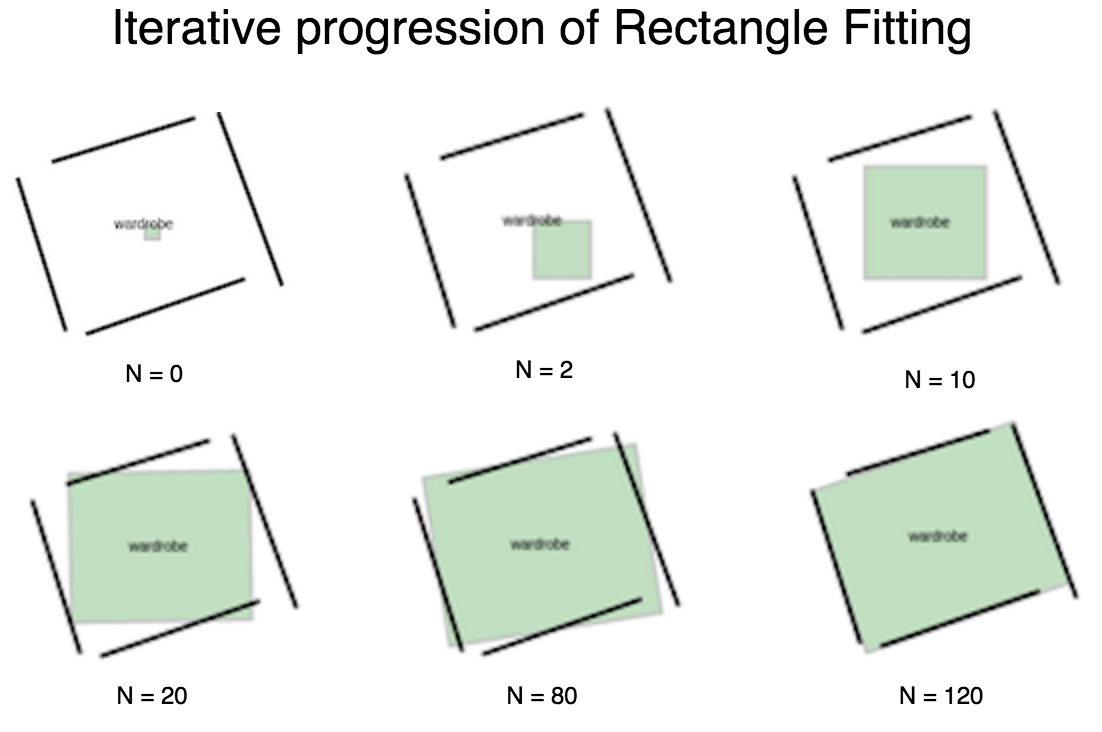
\includegraphics[width=\textwidth]{fitting}
\caption[Iterative step images taken during the rectangle fitting process]{Images taken a different timestamps in the process of iterative fitting.}
\label{fig:fitting}
\end{figure}

After each rectangle created by Algorithm \ref{alg:wiggle} is scored using the before mentioned algorithms, the best scoring iteration is compared to the current iteration. If the new iteration scored better, it becomes the new iteration, and the process repeats. If the current iteration is better, the system has determined that it cannot edit the rectangle any further to create a better scoring result. Therefore, it stops iterating and proceeds to produce a rectangle on the canvas for the user to see. \\

After the rectangle stops iterating, the object has settled in a local minima for score. There is a possibility that it is not the global minima, and that it has settled for a lesser scoring rectangle. Nonetheless, it is acceptable for the rectangle to settle in a local minima since the accuracy is not application breaking. 

\section{Stroke Removal}
\label{sec:strokeremoval}

The removal of strokes presents an interesting problem in this system. As stated in the previous chapter, removal of elements may be done in one of two ways: scribbling and overdrawing. When a stroke is removed by the user, the classifications involving that stroke are no longer valid, as shown in Figure \ref{fig:deleteclass}.

\begin{figure}[ht]
\centering
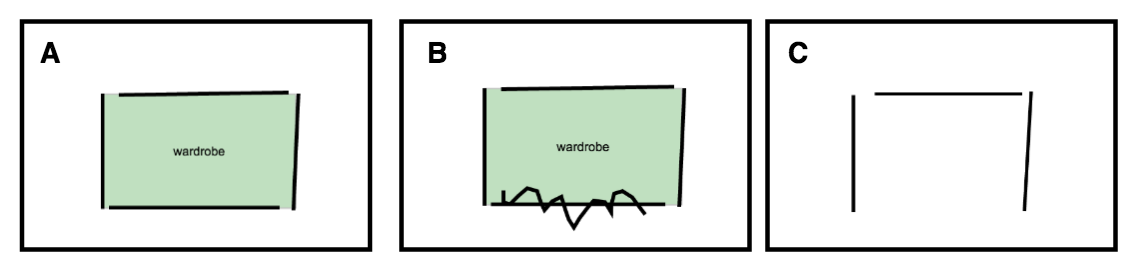
\includegraphics[width=\textwidth]{deleteclass}
\caption[Removal of objects when a stroke is removed]{A diagram depicting the the removal of the object when one of its strokes has been deleted.}
\label{fig:deleteclass}
\end{figure}

As shown in Figure \ref{fig:sketchpipeline}-G, deleting a stroke alters the pipeline slightly. First, the stroke itself must be removed from the interface. Next, all classifications and recognized shapes associated with the removed stroke must also be discarded. If the stroke was not associated with any recognitions, there is no further need to reprocess. However, the removal of those classifications implies that the strokes who used to belong to that recognized object are available. Therefore, we must reprocess the sketch to search for other possible shape recognitions that may be possible.

To start reprocessing the image, stroke combinations are created once again minus the stroke that was removed. The system attempts to readd all strokes that were effected by the removal of one of the strokes. This allows the system to attempt to find new recognized rectangles, if the removed stroke had not existed. Afterwards, the process remains the same as if the process had begun with a new stroke, except using different combinations.

\section{Reclassification}
Furniture items are created via recognition of a viable rectangle present. whose method of creation I will discuss in further detail in the next chapter. However, what will be presented now is the usage of furniture items during sketching, and its available actions and properties.

\begin{figure}[ht]
\centering
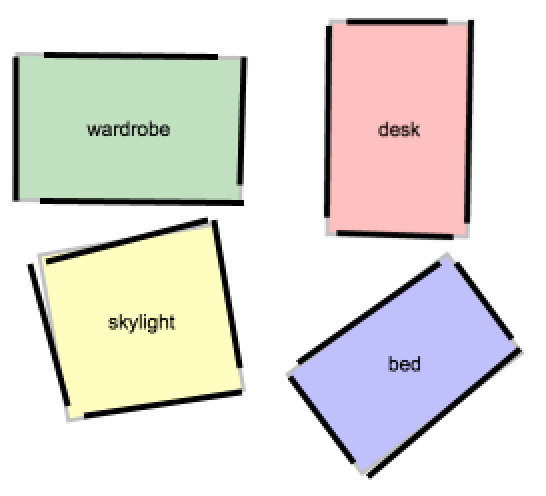
\includegraphics[width=.5\textwidth]{furniture}
\caption[Examples of recognized objects]{Examples of recognized objects. Each piece of furniture or skylight is colored differently, as well as labeled.}
\label{fig:furniture}
\end{figure}

After being recognized, a rectangle is fitted to the strokes. That rectangle may be moved by double clicking and dragging it, also translating its base strokes along to its new location. Objects may not be moved outside the sketching interface boundaries. \\

The rectangle will be assigned an initial classification. Classifications include types of furniture, such as a bed or wardrobe. If the user disagrees with the system's initial classification, the user has two methods of overriding it. First, the user may right-click any object, as shown in Figure \ref{fig:reclassify}, and a menu will appear. The user can reclassify the object as a different object by selecting any of menu items. The only attributes that are modified are the name, type, and color of the object.

\begin{figure}[ht]
\centering
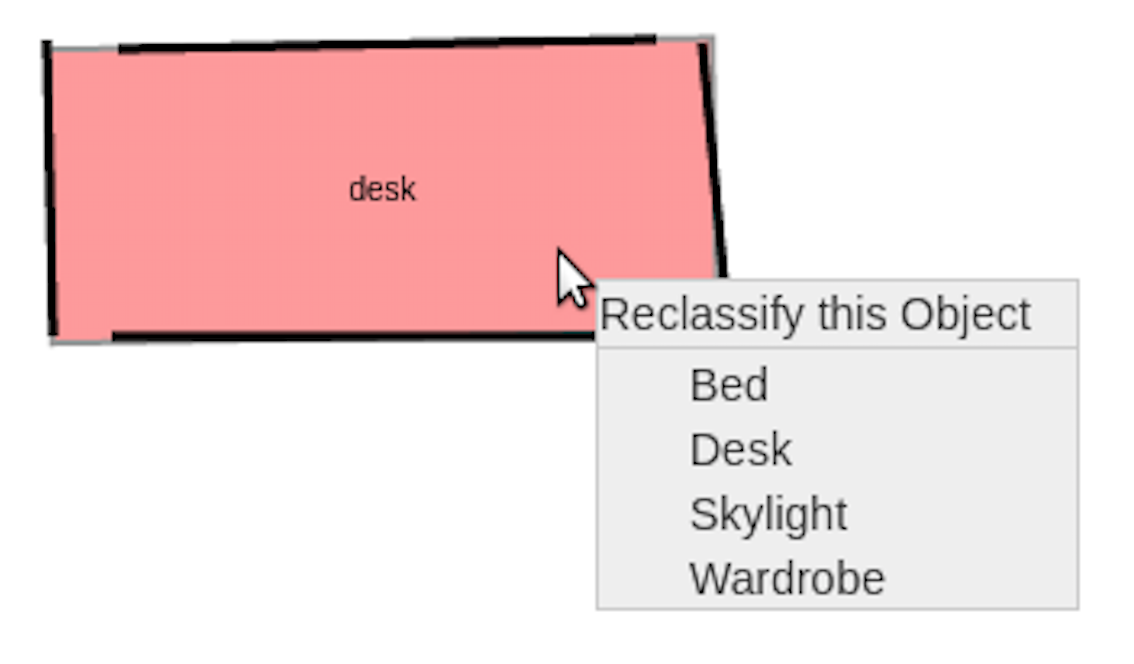
\includegraphics[width=.5\textwidth]{reclassify}
\caption[Image of the reclassification menu]{Upon right clicking on an object, a menu is shown to the user.}
\label{fig:reclassify}
\end{figure}

A second method the user has to reclassify an object is to sketch the corresponding letter on top of the object. The corresponding letter is the first letter of the desired classification, such as the letter 'W' if the user would like to reclassify an object to a wardrobe.

\begin{figure}[ht]
\centering
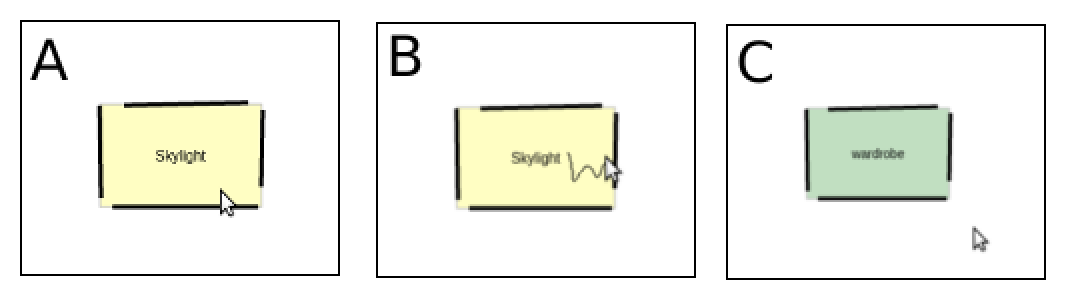
\includegraphics[width=\textwidth]{reclassifydraw}
\caption[Example of reclassification with recognition]{Upon drawing the correct corresponding letter, the user can reclassify an object to another classification.}
\label{fig:reclassifydraw}
\end{figure}

This recognition works by using the \$N recognizer, as described in chapter 2. Using a set of templates corresponding to the first first letters of each of the types of objects, the newly added stroke is processed by the recognizer to check if it matches with any letters. If it is a confident enough match, and the stroke is within the boundaries of an object, then that object is now reclassified to the new type of object. Afterwards, the classification stroke drawn to classify the object is removed and no longer shown. \\

Each method of reclassification has its merits. The right-click menu is more accurate and less reliant on interpretation, since there is no guesswork needed. The letter recognition is arguably faster and intuitive, but has a much larger margin for error. There exists the possibility of the letter not being recognized, or even recognized as the incorrect letter. With the availability of two methods, the user has even more flexibility and choice with his/her designs. 
%reprocessing the image as if that stroke had not been drawn. 

\section{Chapter Summary}
In this chapter, we reviewed how the system selects combinations of strokes to use in the recognizer, and used scoring functions used to determine the existence of a user drawn rectangle. Afterwards, a method of classification based only on stroke dimensions was presented. Finally, I outlined the procedure used to accurately fit a rectangle to a set of user drawn lines. The following chapter discusses the outline and analysis of a brief pilot study based on this system.